%%%%%%%%%%%%%%%%%%%%%%%%%%%%%%%%%%%%%%%%%%%%%%%%%%%%%%%%%%%%%%%%%%%%%%%%
% Preamble
%%%%%%%%%%%%%%%%%%%%%%%%%%%%%%%%%%%%%%%%%%%%%%%%%%%%%%%%%%%%%%%%%%%%%%%%
\documentclass[11pt]{article}
%
% Packages and other includes
% Pagination
\usepackage[letterpaper, margin=0.8in]{geometry}
\usepackage{hyphenat}
\usepackage{multicol,wrapfig}
\hyphenation{Filipp}
%
% Fonts
\usepackage[T1]{fontenc} % best for Western European languages
\usepackage{lmodern} % Latin Modern instead of CM
\usepackage{textcomp} % required to get special symbols
%
% Math
\usepackage{amsmath, amssymb}
\usepackage{braket}
%
% Graphics, floats, tables
\usepackage{graphicx, color, float, array}
%
% Hyperlinks
\usepackage[hidelinks]{hyperref}
%
% Bibliography
\usepackage[style=chem-acs, sorting=none, backend=biber]{biblatex}
\addbibresource{references.bib}
%
% Revision (see Makefile)
%\input{revision.tex}
%
% Definitions and settings
% Paragraph indent and spacing
\setlength{\parskip}{0.4\baselineskip}
\setlength{\parindent}{0in}
%
% Math mode version of "r" column type (requires array package)
\newcolumntype{R}{>{$}r<{$}}
%
% Title, authors, date
%\title{\vspace{-1in}\textbf{Characterizing and visualizing the halogen--$\pi$ interactions
%    between lissoclimides and eukaryotic ribosome using random phase approximation}}
\title{\vspace{-0.8in}\textbf{Within the random phase approximation,
    can noncovalent interactions be visualized and interpreted?}}
\author{\underline{Brian D. Nguyen}, Chris Vanderwal, and Filipp Furche}
\date{}%\vspace{-0.17in}\today}
%
%
%%%%%%%%%%%%%%%%%%%%%%%%%%%%%%%%%%%%%%%%%%%%%%%%%%%%%%%%%%%%%%%%%%%%%%%%
% Main document
%%%%%%%%%%%%%%%%%%%%%%%%%%%%%%%%%%%%%%%%%%%%%%%%%%%%%%%%%%%%%%%%%%%%%%%%
%

\begin{document}

\maketitle
\vspace{-0.25in}
Natural products have been an important source for designing new cancer
drugs over the past several decades.\autocite{Dias12Metabolites2p303,Butler04JNatProd67p2141}
For example, the chlorolissoclimide (CL) extracted from the ascidian
\textit{Lissoclinum voeltzkowi} is a powerful cytotoxic bicyclic diterpene
alkaloid that inhibits eukaryotic translation elongation.\autocite{Robert06RNA12p717}
This inhibition leads to ribosome accumulation and eventual cell death. 
The X-ray co-crystal structure of CL with the eukaryotic 80S ribosome revealed
a novel halogen--$\pi$ interaction between the ligand's alkyl chloride and two
guanine nucleotides.\autocite{Imai08ProteinScience17p1129,Konst2017} This
type of interaction has been noted to be dispersion
dominant.\autocite{Riley08JChemTheoryComput4p232,Riley13PhysChemChemPhys15p17742,
  Sedlak14JPhysChemA118p3846} In this research project, I will combine both
experimental and theoretical methods to tune dispersion interactions for
designing and synthesizing analogues of lissoclimide for new cancer
therapeutics.

To achieve the project's goal, the correct computational and theoretical understanding of
dispersion interactions are key to designing new therapeutics. Dispersion is not
only non-trivial to predict computationally but also, it is even harder to
characterize and interpret. In a recent publication, we demonstrated that
the random phase approximation (RPA) provides the correct description of dispersion
interactions compared to the many-body perturbation theory (MBPT) for noncovalent
interactions (NIs).\autocite{Nguyen20JChemTheoryComput16p2258} The accuracy of RPA
is achieved without any additional empirical parameters and at an efficient
computational cost. Based on this study, I propose using RPA to develop a
visualization tool for characterizing dispersion interactions that can then be
applied to a simplified model of the intermolecular interactions between
the CL and eukaryotic 80S ribosome, see Fig. \ref{fig:model}.

\begin{wrapfigure}{r}{0.5\linewidth}
  \vspace{-33pt}
  \centering
  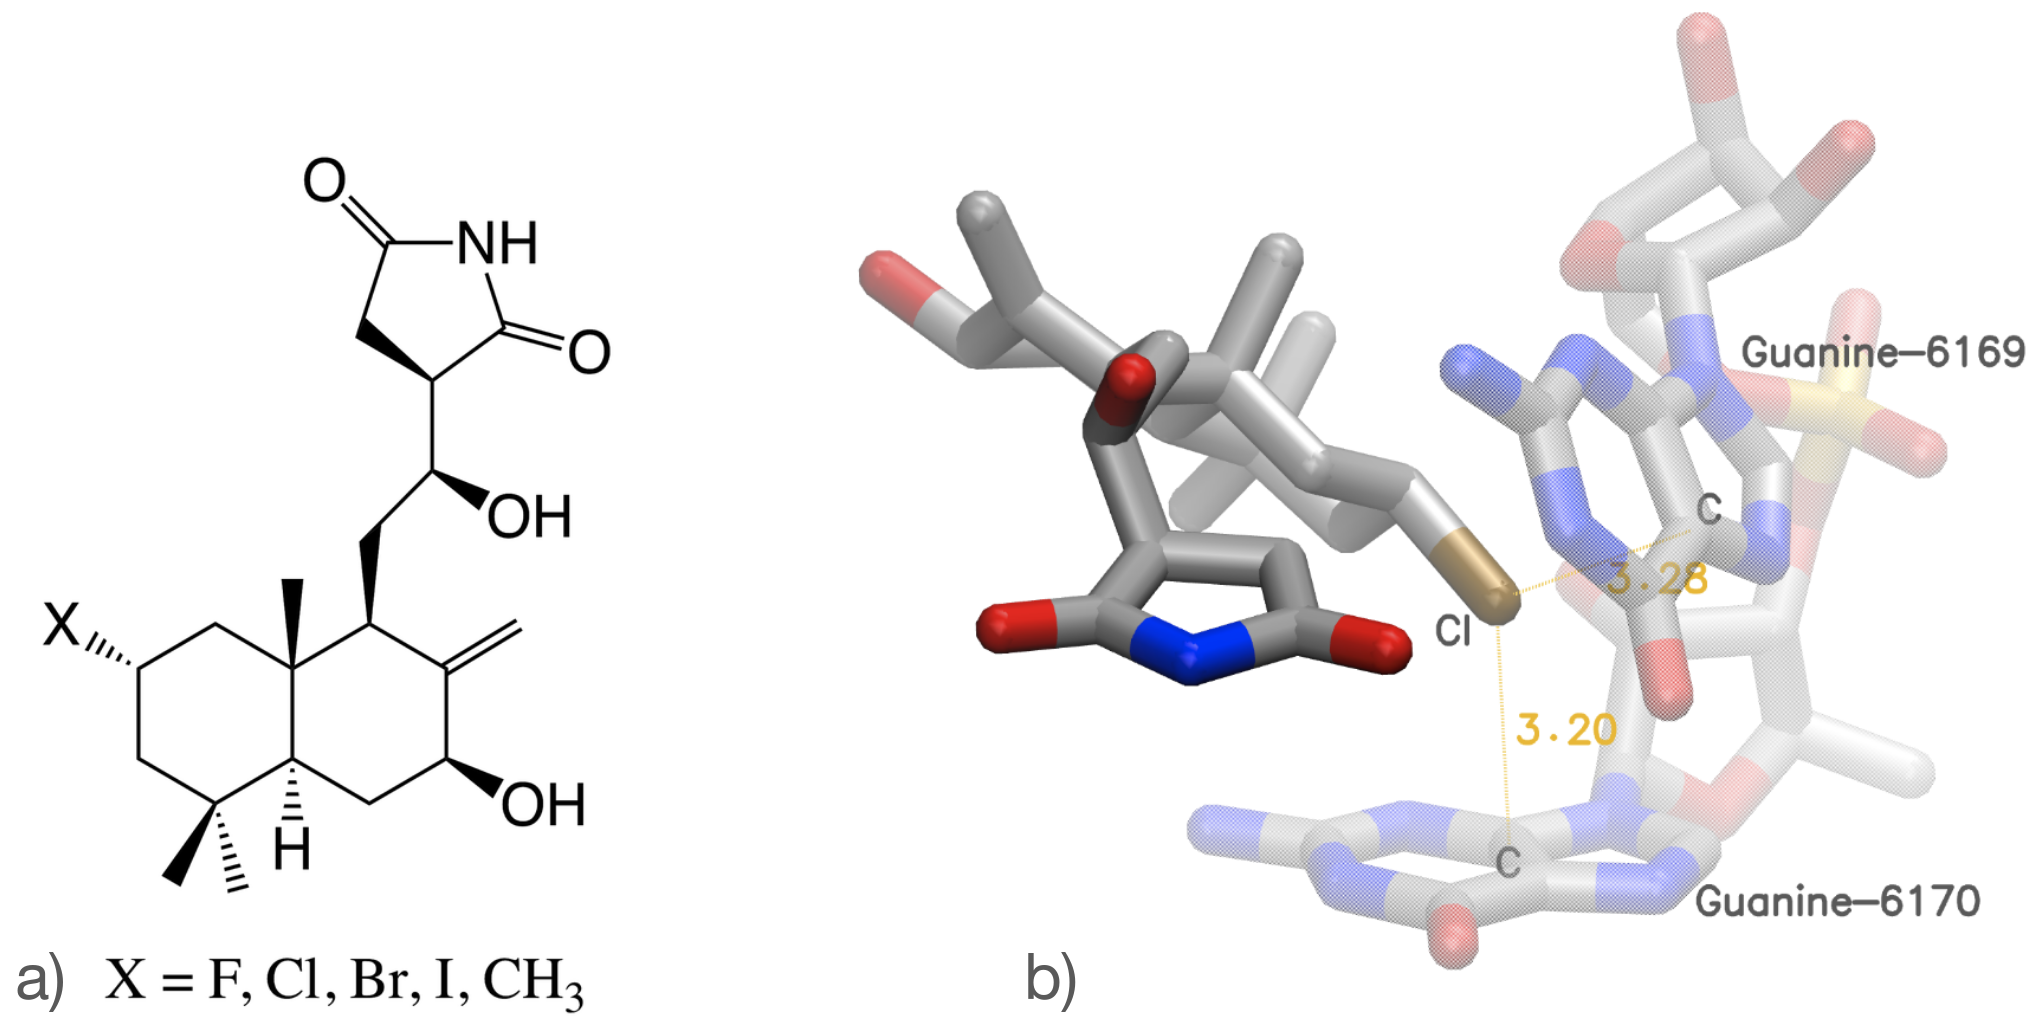
\includegraphics[scale=0.12]{combined.png}
  \caption{a) A series of substituted lissoclimides of different halogens.
    b) Geometry optimized model of CL and guanine nucleotides using the hybrid
    density functional TPSSh-D3.\autocite{Staroverov03JChemPhys119p12129,Grimme12ChemEurJ18p9955}
    Bond lengths are in Angstroms. Hydrogens were removed for clarity. Color codes
    for atoms are Cl = brown, N = blue, C = gray, O = red, and P = orange.\vspace{-11pt}}
  \label{fig:model}
\end{wrapfigure}

I will be coordinating with my primary advisor Filipp Furche in
theoretical chemistry and my secondary advisor Chris Vanderwal in organic
chemistry to elucidate the behaviors of NIs and then apply these predictions
to design better cancer therapeutics. The research plan consists of three
parts where the first two parts are done in the Furche Group while the third
part is performed in the Vanderwal Group.

First, I will conduct a comprehensive computational study on the nature
and magnitude of the intermolecular interaction by varying the halogen
moiety (X = F, Cl, Br, I, CH$_3$) as an extension to the work by K{\"o}nst
\textit{et al.},\autocite{Konst2017} see Fig. \ref{fig:model}. My preliminary
gas phase binding energies for the lissoclimide family were shown to increase
going down the halogen group. However, the question of why this trend
is observed remains. To explain this observation, I will develop a visualization
tool for dispersion interactions by interpreting the corresponding eigenvectors of
the RPA correlation energies as plasmonic modes describing collective excitations
of the electrons. Lastly, the third part is the confirmation of the computational
results by synthesis of the substituted lissoclimide along with testing
the drug's potency through \textit{in vitro} studies.

For my doctoral studies, I have envisioned my dissertation
to be focused on developing state-of-the-art approaches that accurately
describe NIs. We have concluded from our recent landmark publication that
RPA with its superior accuracy for NIs may safely replace MBPT for predictions
of NIs in most systems of chemical interest.\autocite{Nguyen20JChemTheoryComput16p2258}
With this research project, I will be able to apply diverse skills from
organic synthesis and theoretical chemistry to develop RPA based methods
that interpret NIs relevant for drug design.

\printbibliography

\end{document}
